
\section{Results and Discussion}\label{sec:results}

In this section, we present and discuss the results related to providing mFRR versus load shifting for a single supermarket freezer using the optimization model in (\ref{P1:compact_model}), and the scenarios and solution strategies described in Section \ref{sec:scenario_generation} and \ref{sec:mFRR_bidding_implementation}. First, we discuss the main result: mFRR versus load shifting. Second, we discuss the effectiveness of the ADMM solution strategy using 2021 price data.

\subsection{Load shifting vs mFRR}

Figure \ref{fig:cumulative_cost_comparison} shows the cumulative cost of operation for mFRR versus load shifting compared to the baseline cost. For mFRR, the lookback strategy is similar to ADMM strategy using 2021 scenarios. But both of them have a higher cost than load shifting for most of the year. Interestingly, mFRR was very profitable in June (reservation prices increased significantly due to an outage of a reserve power plant).

\begin{figure}[!t]
    \centering
    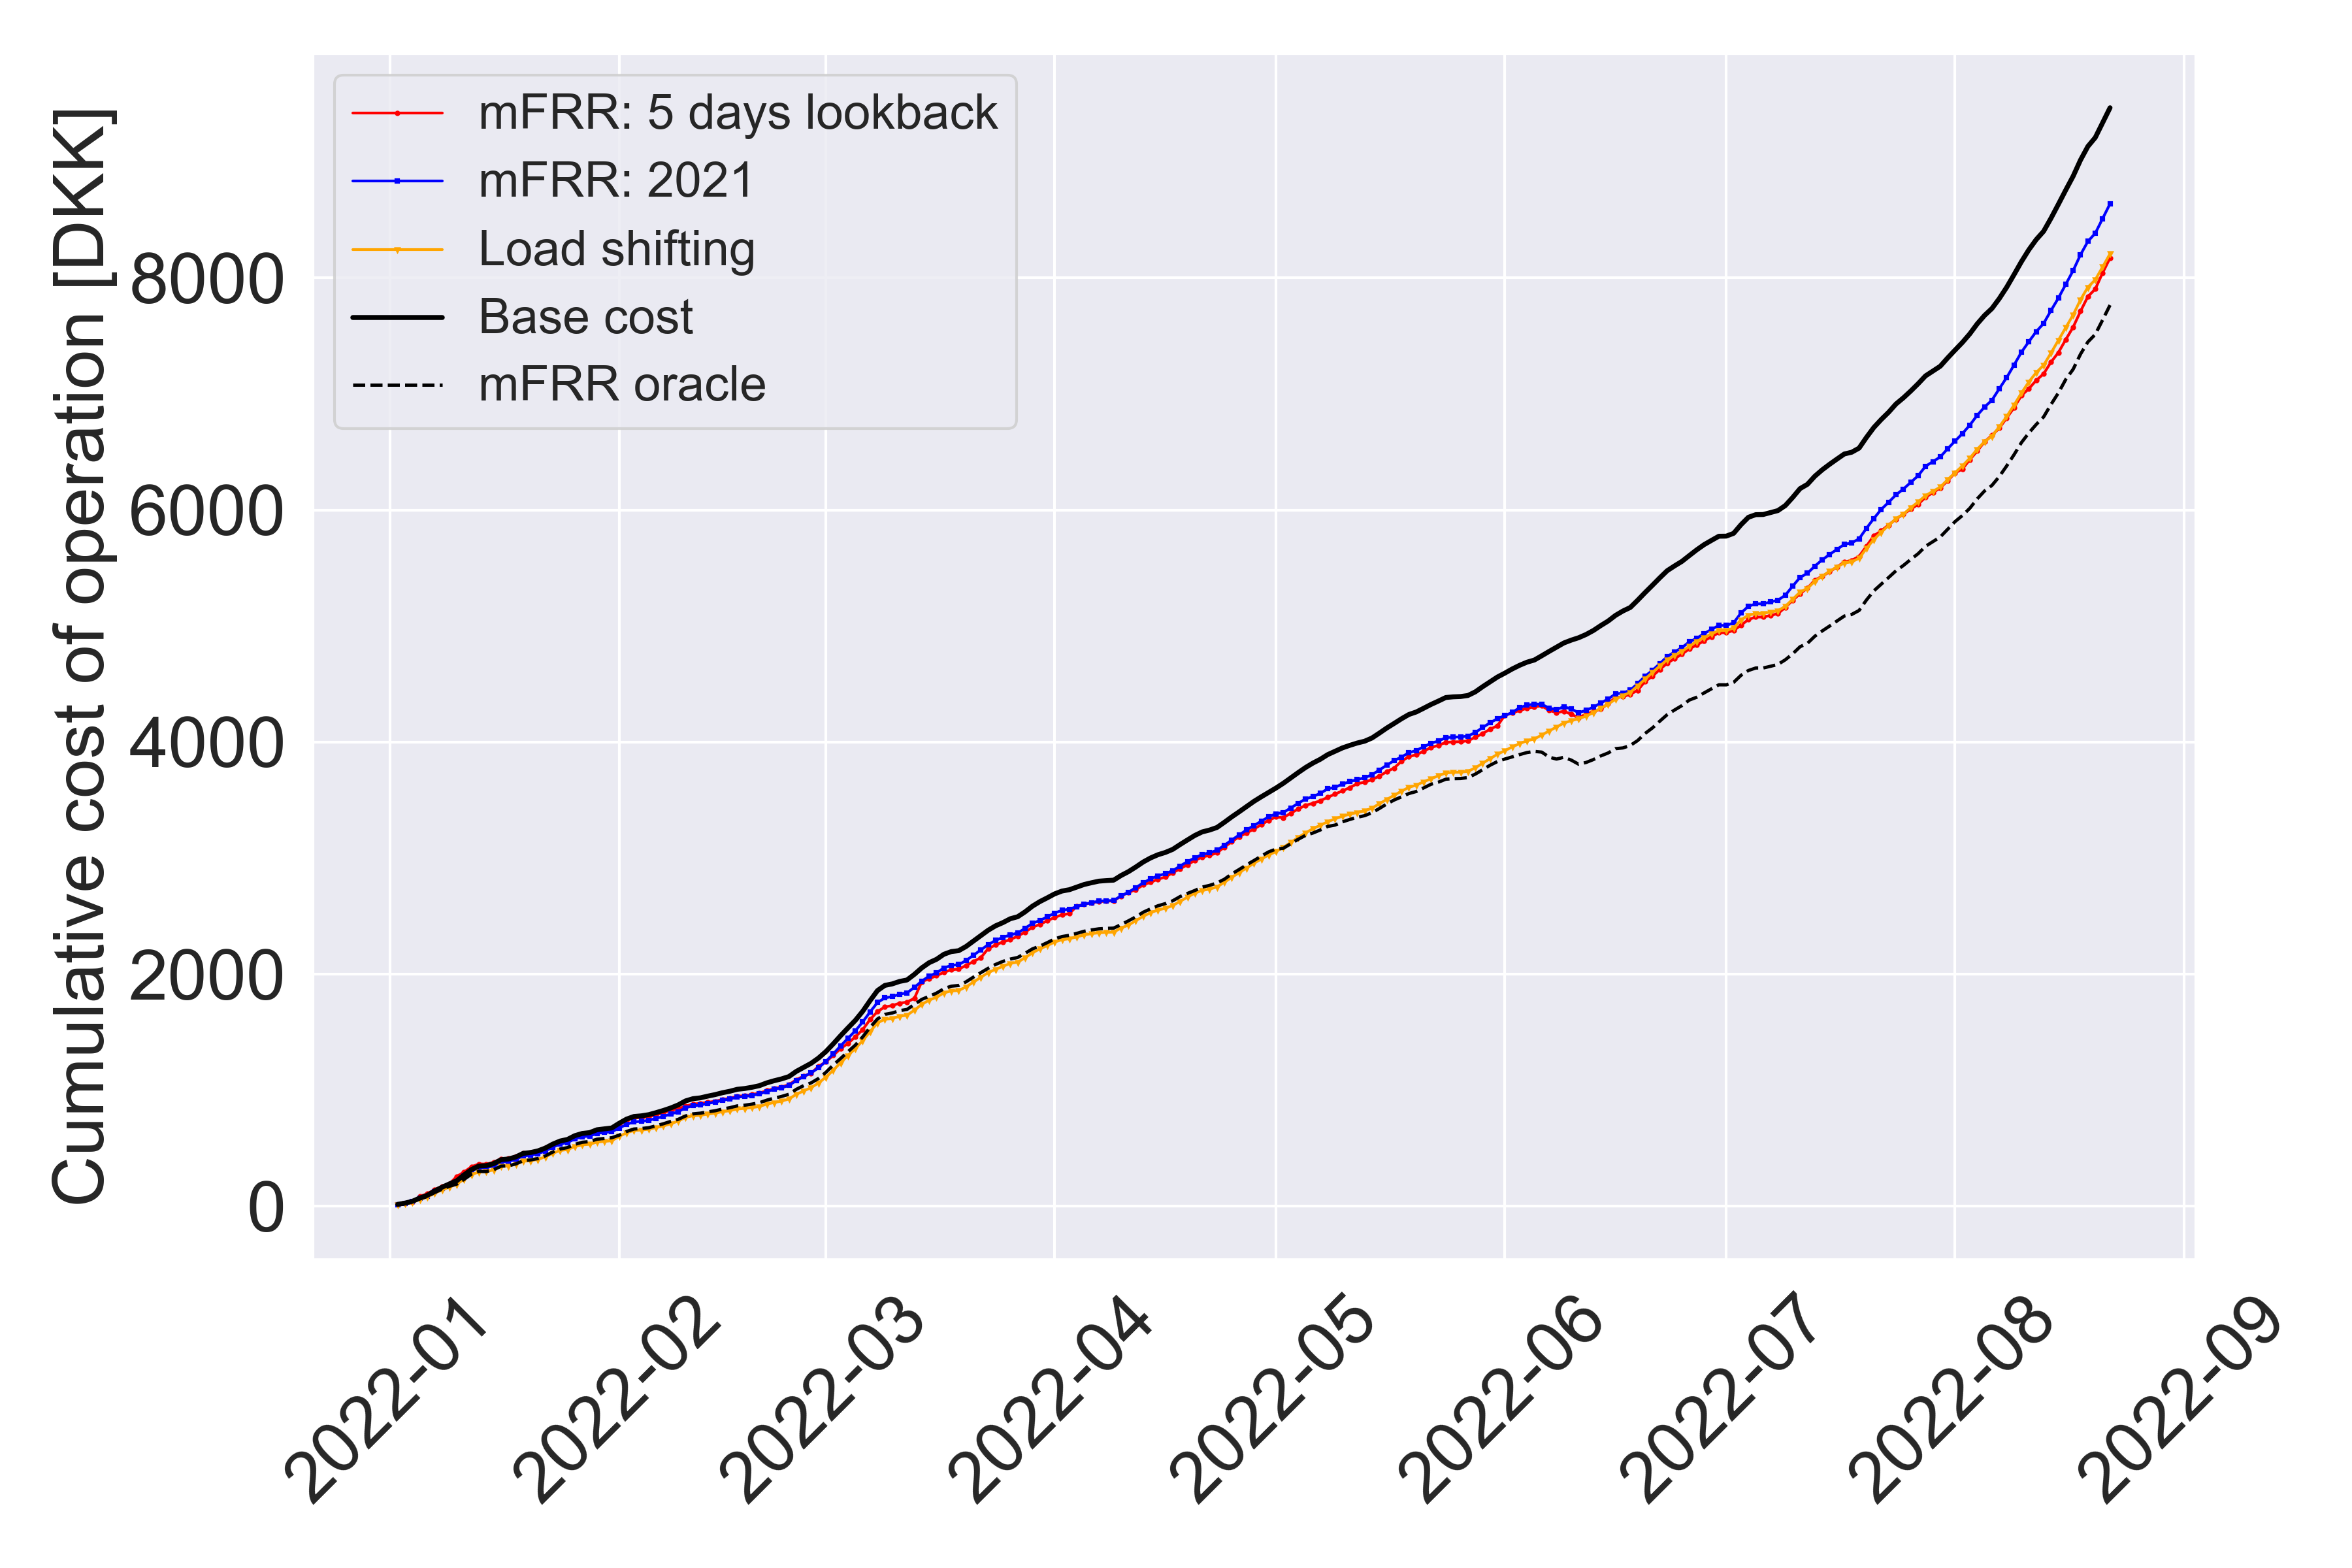
\includegraphics[width=\columnwidth]{../figures/cumulative_cost_comparison.png}
    \caption{OOS cumulative cost of operation for load shifting and mFRR using ADMM with 50 scenarios trained on 2021 data (blue), and a lookback of five days (red). Base costs are also shown together with an oracle that has full hindsight on prices.}
    \label{fig:cumulative_cost_comparison}
\end{figure}

Table \ref{tab:cases_compared} breaks down the cost components. For mFRR, there is big difference between the lookback strategy and the ADMM strategy with 2021 prices. The lookback strategy earns much more from activation payments, but is also penalized more as it is not able to deliver its reservation capacity in some days. The other mFRR strategy bids more conservatively and is only rarely activated. The market rules prescribe that the full bid should be delivered, hence the lookback strategy might be too risky. On the other hand, it was assumed that the activation power should be equal to the reserved power, but the TSO determines the activation power, hence the activation power might be lower in reality which would both decrease the penalty cost and the activation revenue.

All strategies are better than the baseline costs, i.e., not utilizing flexibility, with savings of 10-14\%. Furthermore, the mFRR strategies are not far off the theoretically best mFRR strategy as indicated by the oracle in Figure \ref{fig:cumulative_cost_comparison}.

\begin{flushleft}
    \begin{table}[!t]
        \caption{Average Daily OOS Costs.}
        \label{tab:cases_compared}
        \centering
        \begin{tabular}{lccc}
            \toprule
            Name                 & \thead{mFRR w.                   \\lookback} & Load shifting & \thead{mFRR \\w. 2021} \\
            \midrule
            Base cost today      & 40.628         & 40.628 & 40.628 \\
            Total cost           & 35.918         & 34.994 & 36.514 \\
            Expected energy cost & 40.628         & 34.994 & 40.628 \\
            Rebound cost         & 0.858          & N/A    & 0.911  \\
            Reserve payment      & 3.216          & 0.0    & 3.381  \\
            Act payment          & 8.092          & 0.0    & 2.161  \\
            Penalty cost         & 5.741          & 0.0    & 0.516  \\
            Scenarios            & -5             & 1      & 50     \\
            ADMM                 & False          & False  & True   \\
            \% savings           & 11.6           & 13.9   & 10.1   \\
            \bottomrule
        \end{tabular}
    \end{table}
\end{flushleft}

In Figure \ref{fig:fig_sim}, load shifting and mFRR are compared for the same day. For load shifting, it can clearly be seen how load is shifted to low-price hours, especially at the end of the day. But it also has a very significant effect on the temperature with large deviations from its normal setpoint. For mFRR, the reservation is almost full for all hours during the day. The activation of reservation occurs when the bid price is lower than the balancing price which in this particular scenario only happens for three hours. The effect on the temperature is therefore much smaller than for load shifting. The model is also able to rebound smartly in hour 19 to avoid high rebound costs.

\begin{figure*}[!t]
    \centering
    \subfloat[]{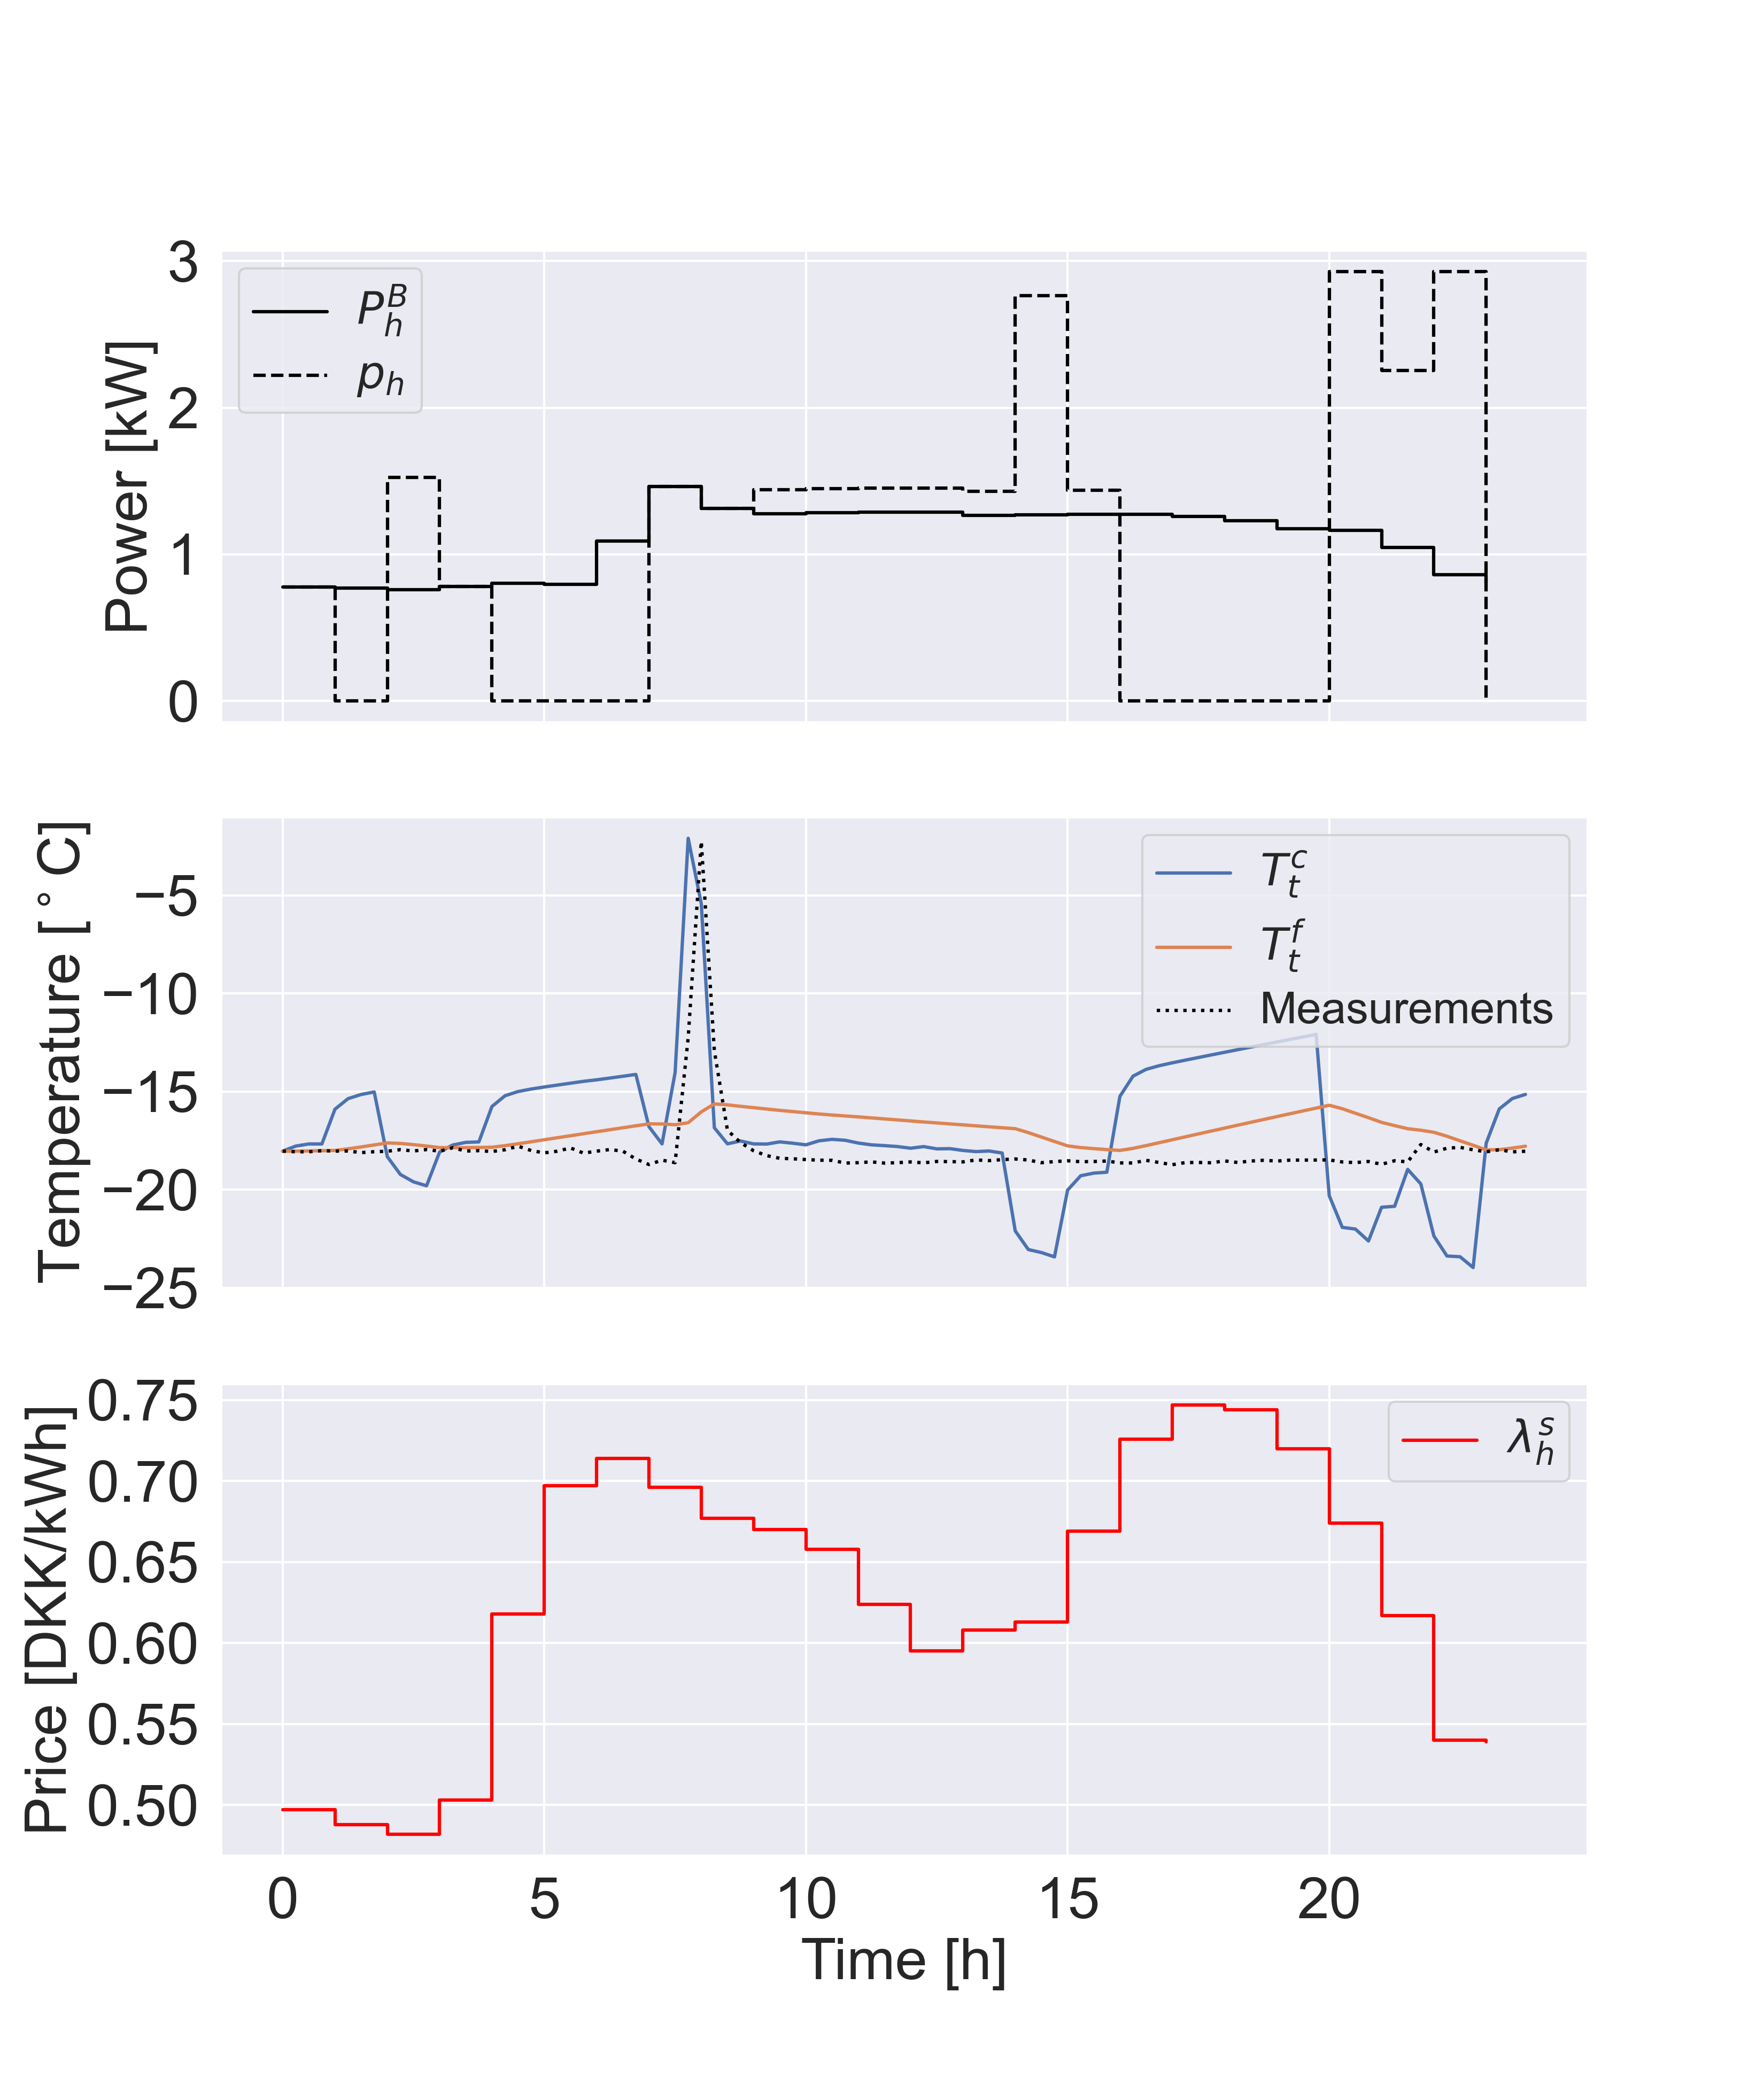
\includegraphics[width=\columnwidth]{../figures/spot_single_case.png}%
        \label{fig_first_case}}
    \hfil
    \subfloat[]{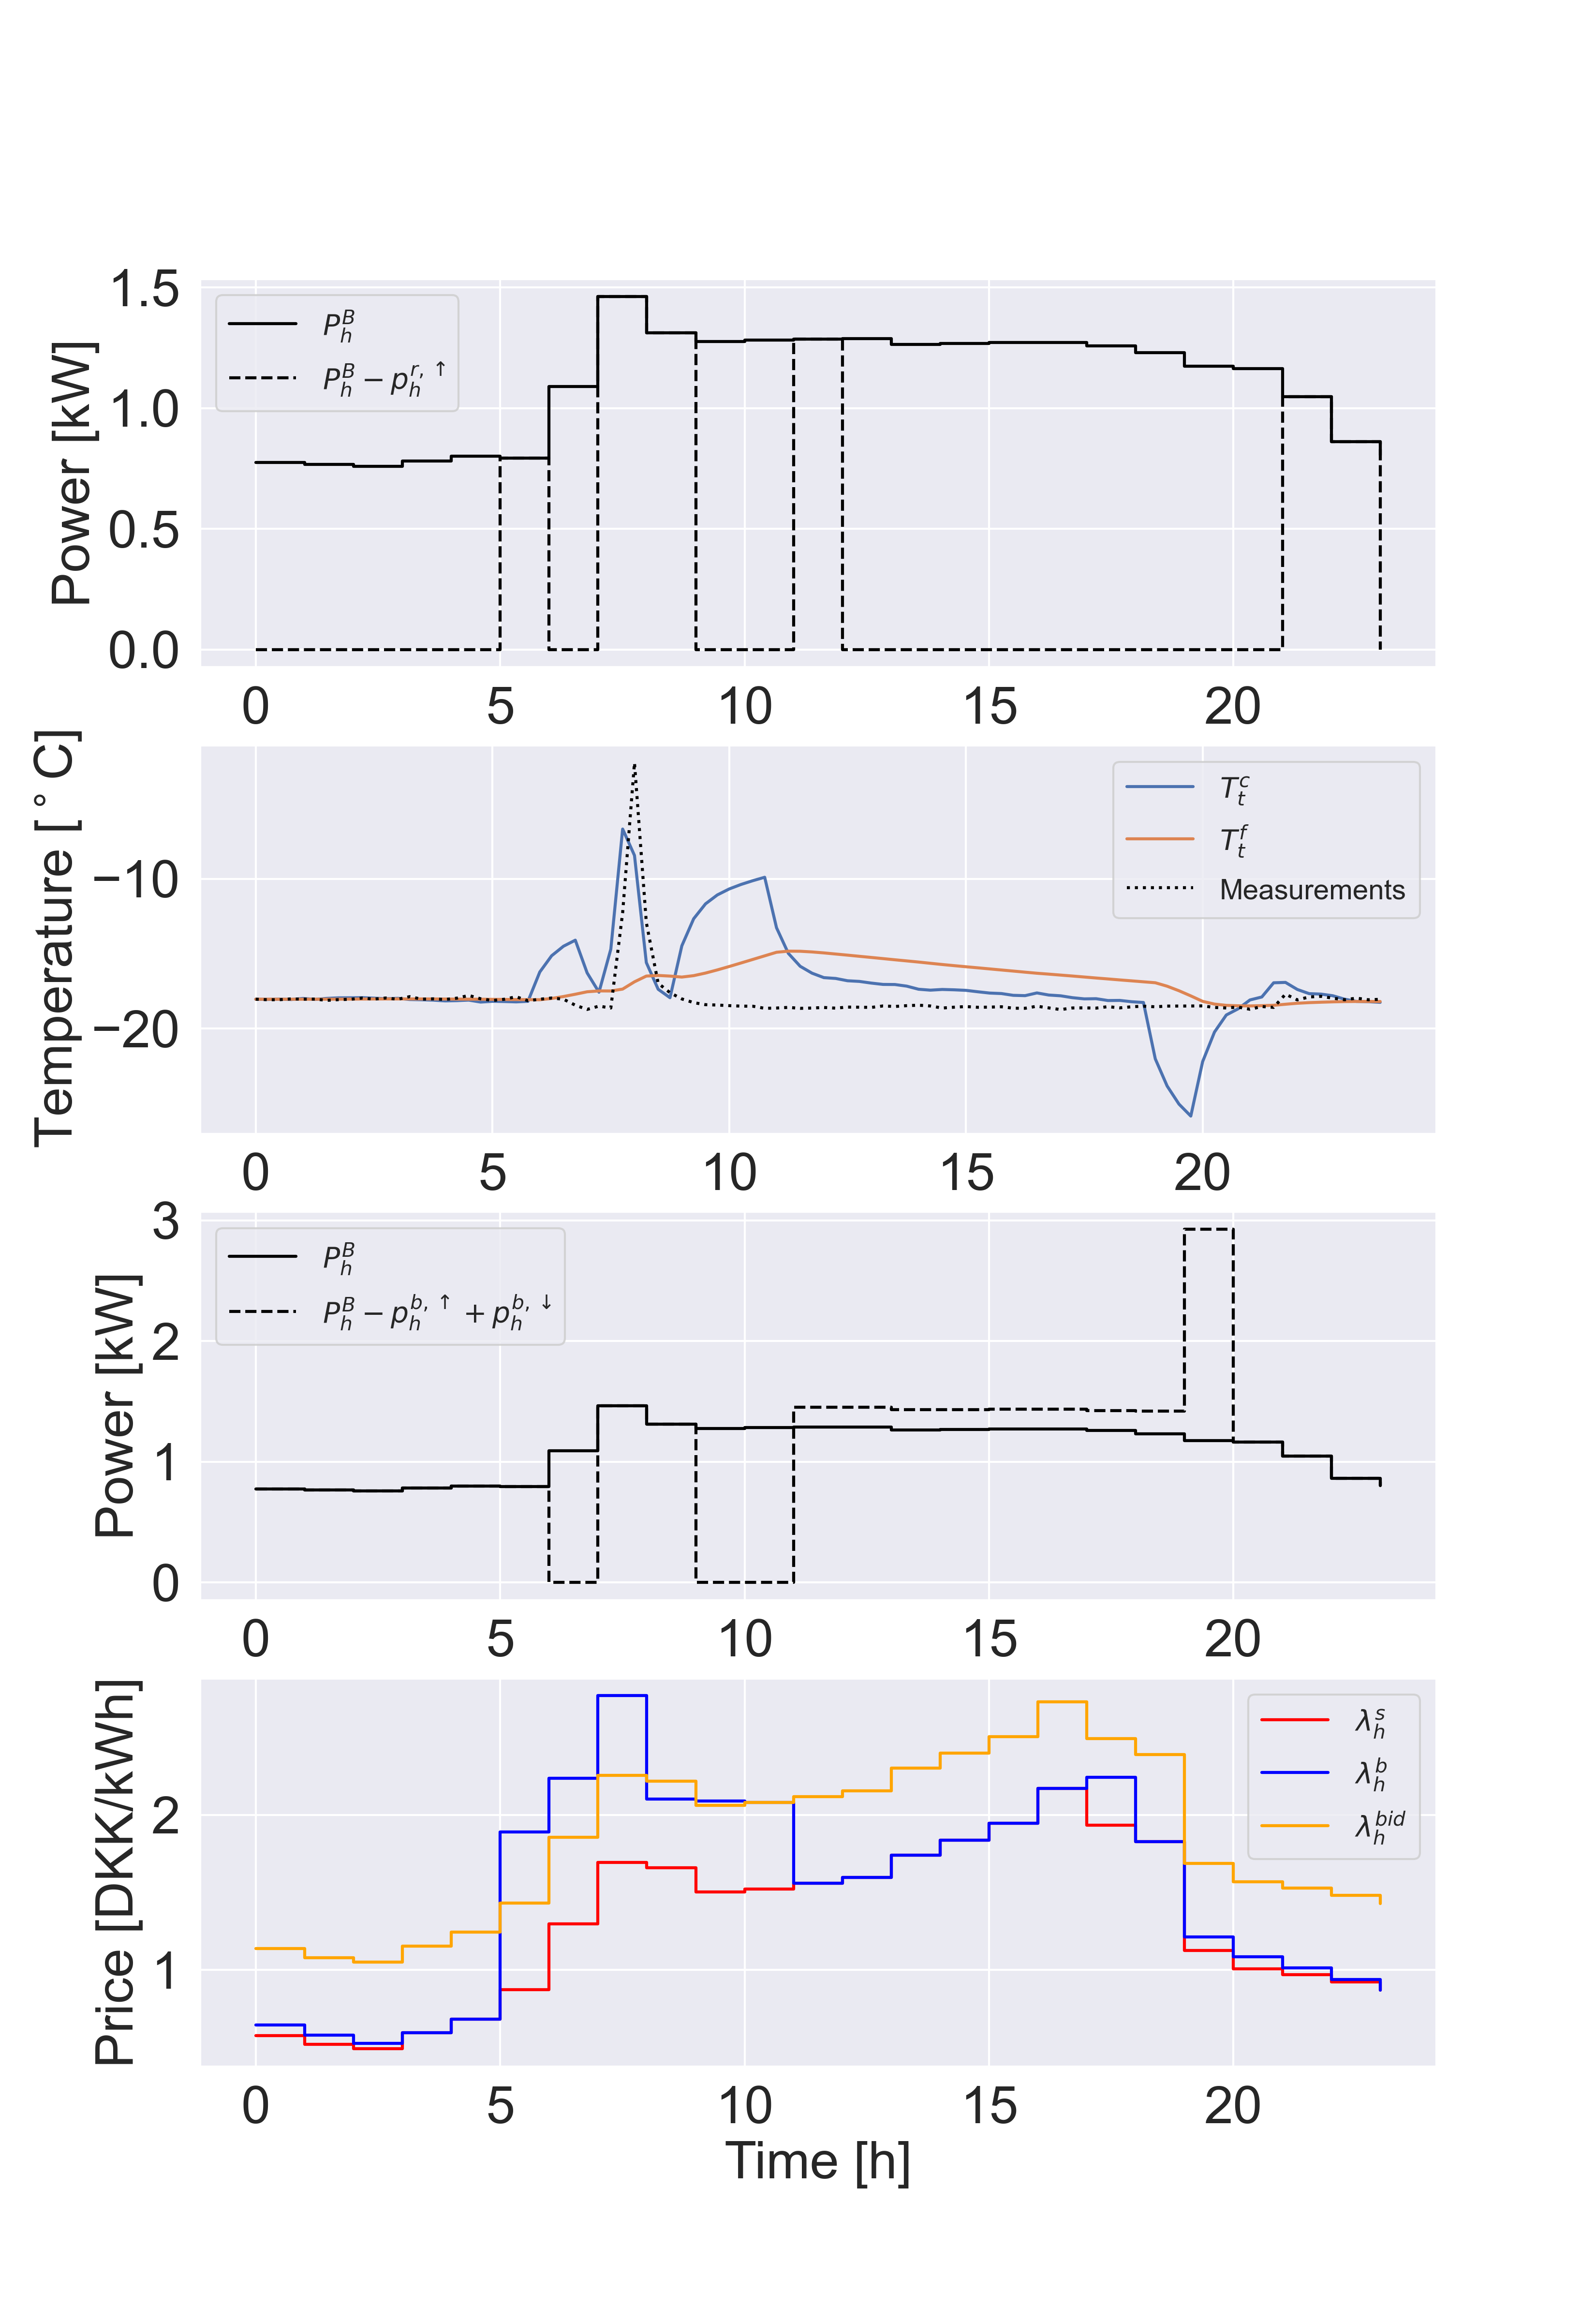
\includegraphics[width=\columnwidth]{../figures/mFRR_single_case.png}%
        \label{fig_second_case}}
    \caption{Comparison between load shifting and mFRR in one IS scenario. \textbf{a}: \textbf{Top}: Power profile when load shifting and baseline power of freezer. \textbf{Middle}: Air and food temperature dynamics. \textbf{Bottom}: Spot price in scenario. \textbf{b}: \textbf{Top}: Reservation capacities and baseline power of freezer. \textbf{Upper middle}: Air and food temperature dynamics. \textbf{Lower Middle}: mFRR activations in this scenarios, i.e., when $\lambda_{h}^{bid} \leq \lambda_{h}^{b}$, $\lambda_{h}^{b} > \lambda_{h}^{s}$ and $p^{r,\uparrow}_{h} > 0$. \textbf{Bottom}: Spot price, balancing price, and bid price in scenario.}
    \label{fig:fig_sim}
\end{figure*}

The results show some interesting features of mFRR and load shifting. Although the savings are higher for load shifting, they are directly proportional to the energy shifted and therefore the temperature deviation in the freezer. For mFRR, this is not the case due to the mechanism of reservation and activation.

Furthermore, settlement costs of the BRP for load shifting were ignored as this reflects the reality of selfish, flexible consumers acting in their own interest. In reality, the BRP would have to pay for the settlement costs or at least buy/sell energy in the intraday market after the day-ahead market clearing and load shifting schedule. But consumers are not necessarily aware of the balance settlement and the electricity market mechanisms. Hence, they have a strong incentive to use their flexibility for load shifting. Some industrial and commercial consumers might not be exposed fully to the spot price, and for those consumers, load shifting is less profitable, but they will still have an incentive to change their deal with the retailer to get full exposure.

For mFRR, it was implicitly assumed that all revenue from reservation and payments go to the flexible consumer. But this neglect the fact that the BRP requires a share of the revenue. Furthermore, there might be an aggregator or technology provider facilitating the aggregation and communication of the flexibility. In this case, the they would also want a share of the revenue. This can potentially reduce the revenue of the consumer significantly and is one of the main challenges of achieving widespread penetration of demand-side flexibility \cite{gade2022ecosystem}.

As mentioned, a single freezer or supermarket must be part of a larger portfolio through an aggregator in order to participate in mFRR. Such an aggregated portfolio has some issues that are neglected here, such as baseline estimation for verification of the demand response, allocation of profits within the portfolio, and accurate capacity estimation of the whole portfolio that bid into mFRR.

Furthermore, mFRR is changing from a 60-min market to a 15-min market in the next few years \cite{MARI}. This makes it more feasible for TCLs to participate given their sensitivity to large temperature deviations.

Nevertheless, load shifting seems more appealing for a flexible consumer compared to mFRR from a monetary point of view. This finding illustrates the importance of designing attractive markets for mFRR if demand-side flexibility is to be used more widely, and perhaps also to disincentivize load shifting for flexible consumers as it could lead to system imbalances.


\subsection{ADMM}

Figure \ref{fig:admm_vs_normal_solution} shows the ADMM convergence to the optimal solution for five scenarios for different step sizes. For most step sizes, it converges quickly but never quite reaches the optimal solution. This is mainly because the algorithm has to achieve consensus on three variables, $p_{h,\omega}^{r,\uparrow}$, $\alpha_{\omega}$, and $\beta_{\omega}$. Experiments showed that it was converging much closer to the optimal solution when removing $\alpha_{\omega}$, and $\beta_{\omega}$.

A large step size emphasizes the need to reach consensus whereas a small step size prioritizes the objective function in (\ref{P1:eq1}). Here, it seems a step size of $\gamma \geq 1$ is more stable and converges quickly.

\begin{figure}[!t]
    \centering
    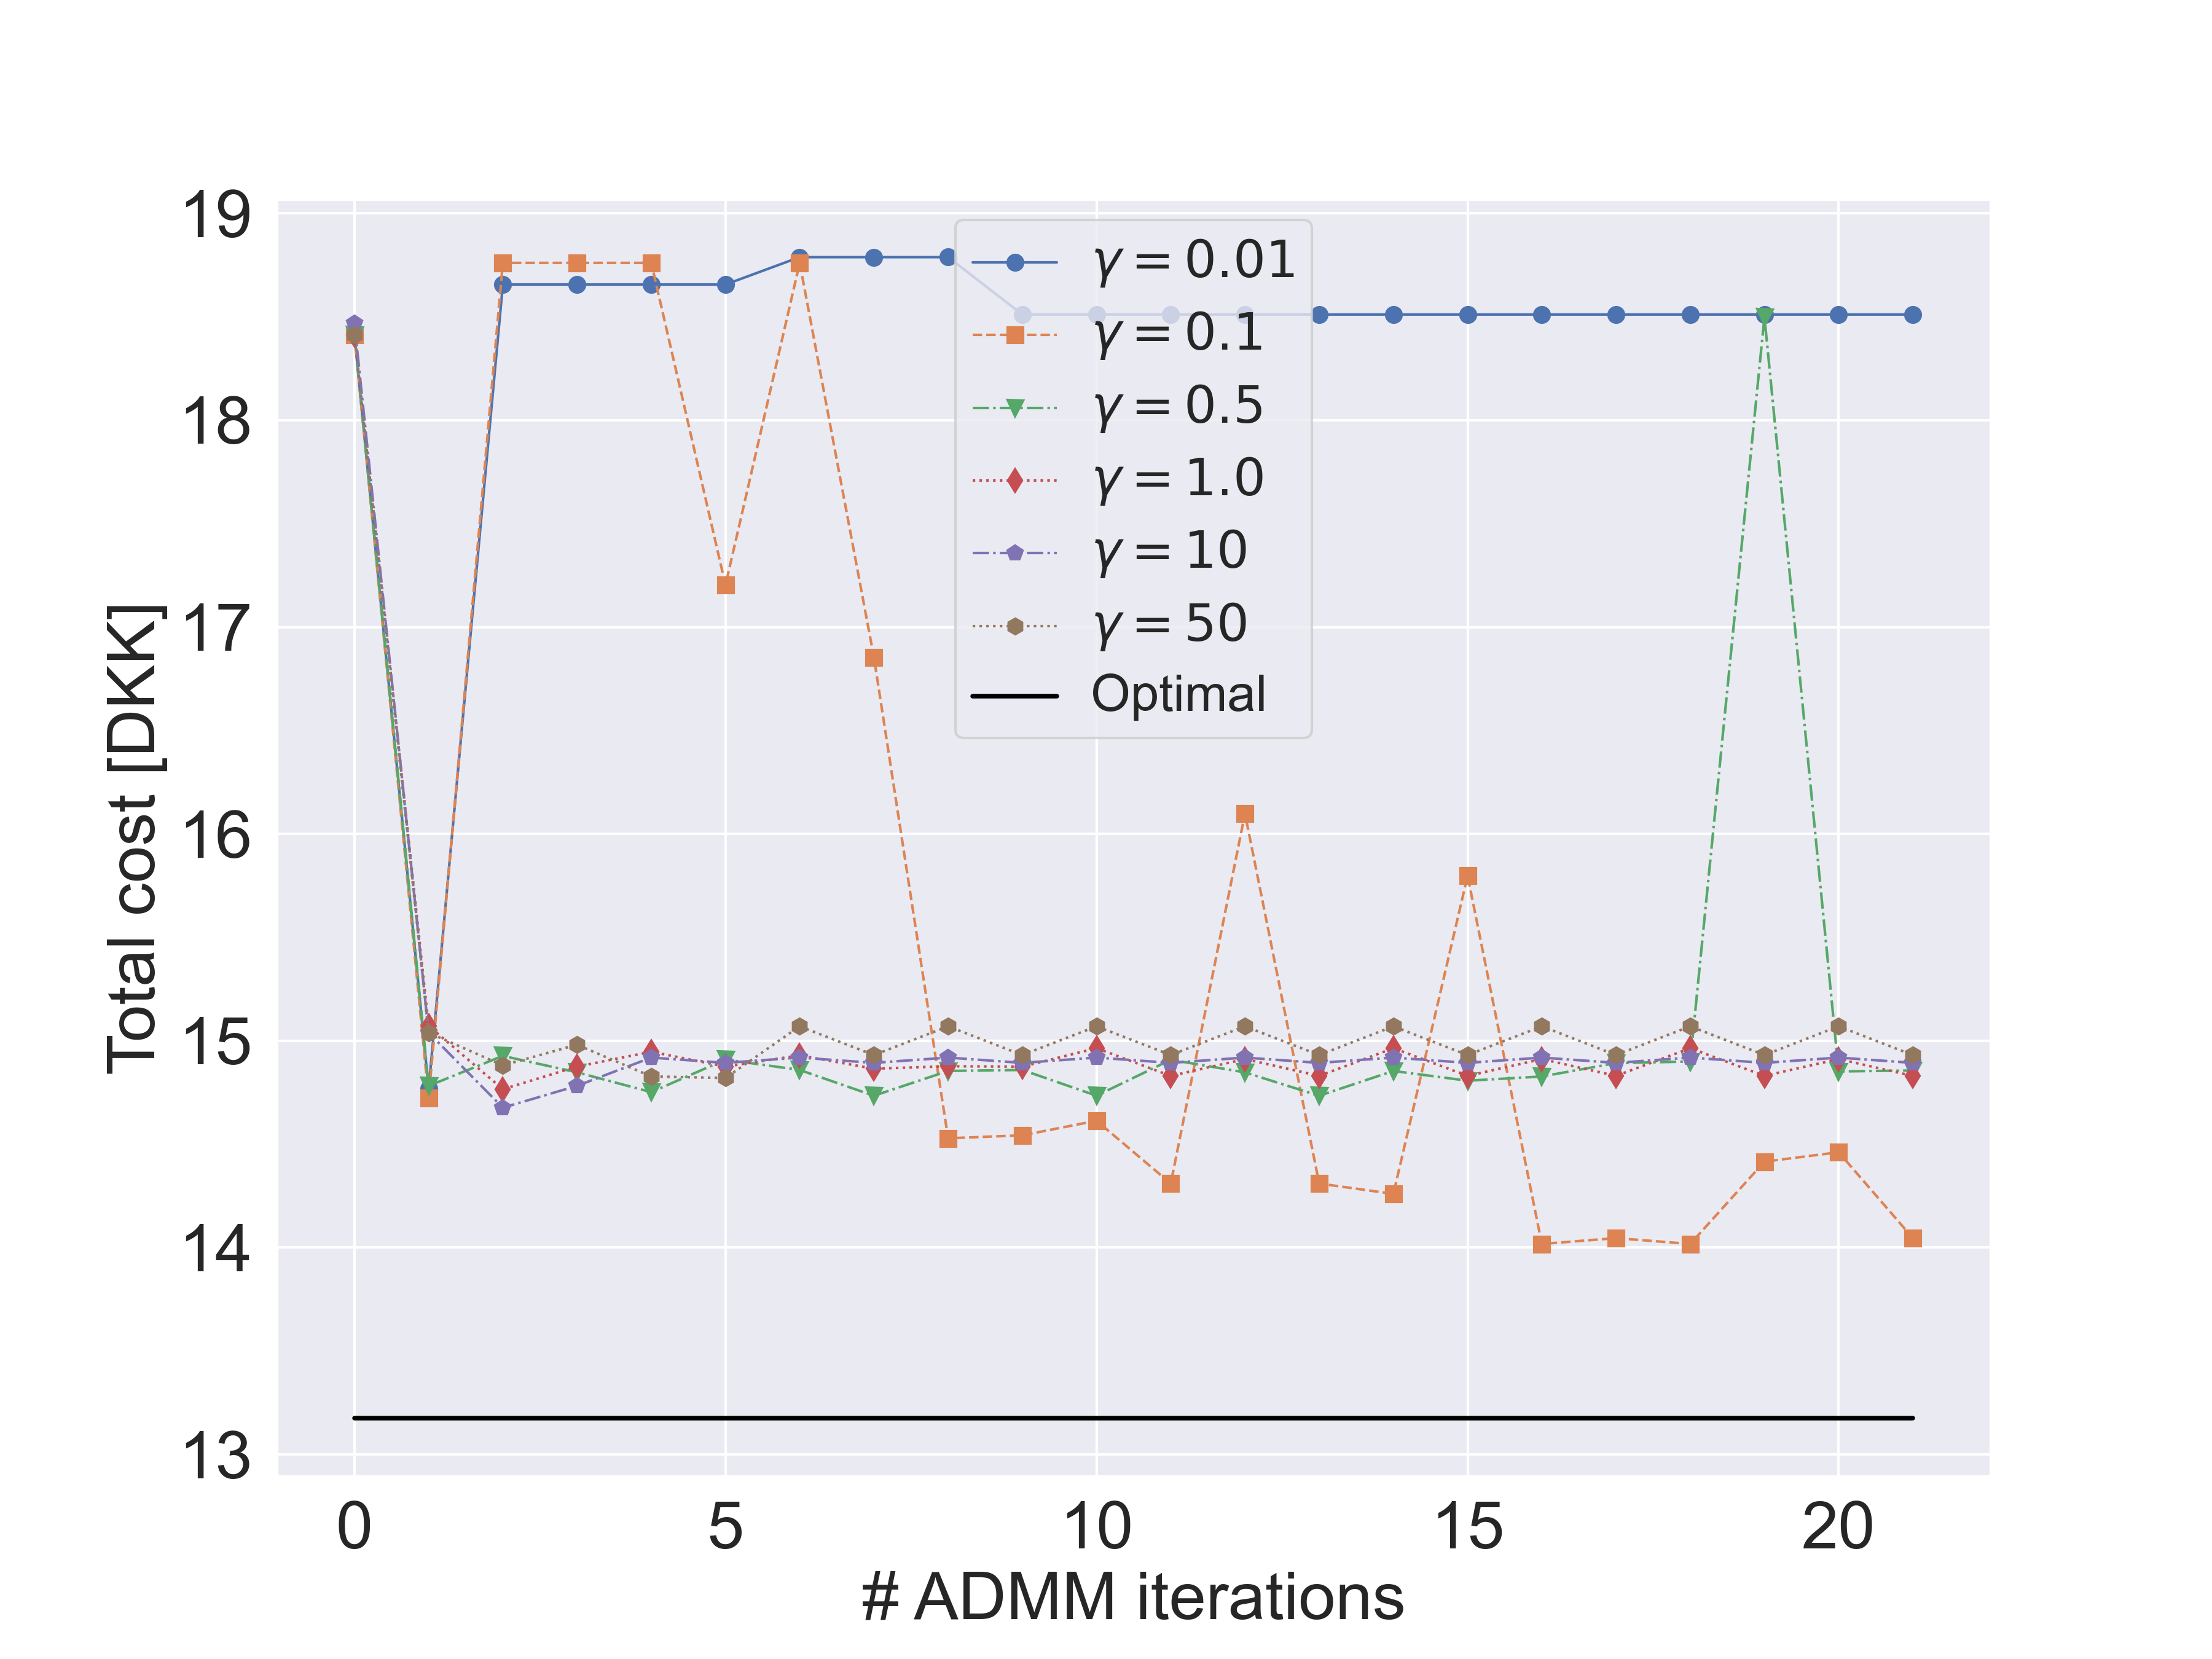
\includegraphics[width=\columnwidth]{../figures/admm_vs_normal_solution.png}
    \caption{ADMM solution versus the optimal solution for five scenarios for different step sizes in the ADMM algorithm.}
    \label{fig:admm_vs_normal_solution}
\end{figure}

Figure \ref{fig:admm_nb_scenarios_effect} shows the effect of including more scenarios in Problem (\ref{P1:compact_model}) using ADMM to solve it. For IS, good solutions are already obtained with 5-10 scenarios, and the same applies for OOS although it seems using 250 scenarios also performs well.

The plot highlights the importance of choosing representative scenarios, especially balancing prices as they determine how much activation is needed, and therefore the bid policy.

\begin{figure}[!t]
    \centering
    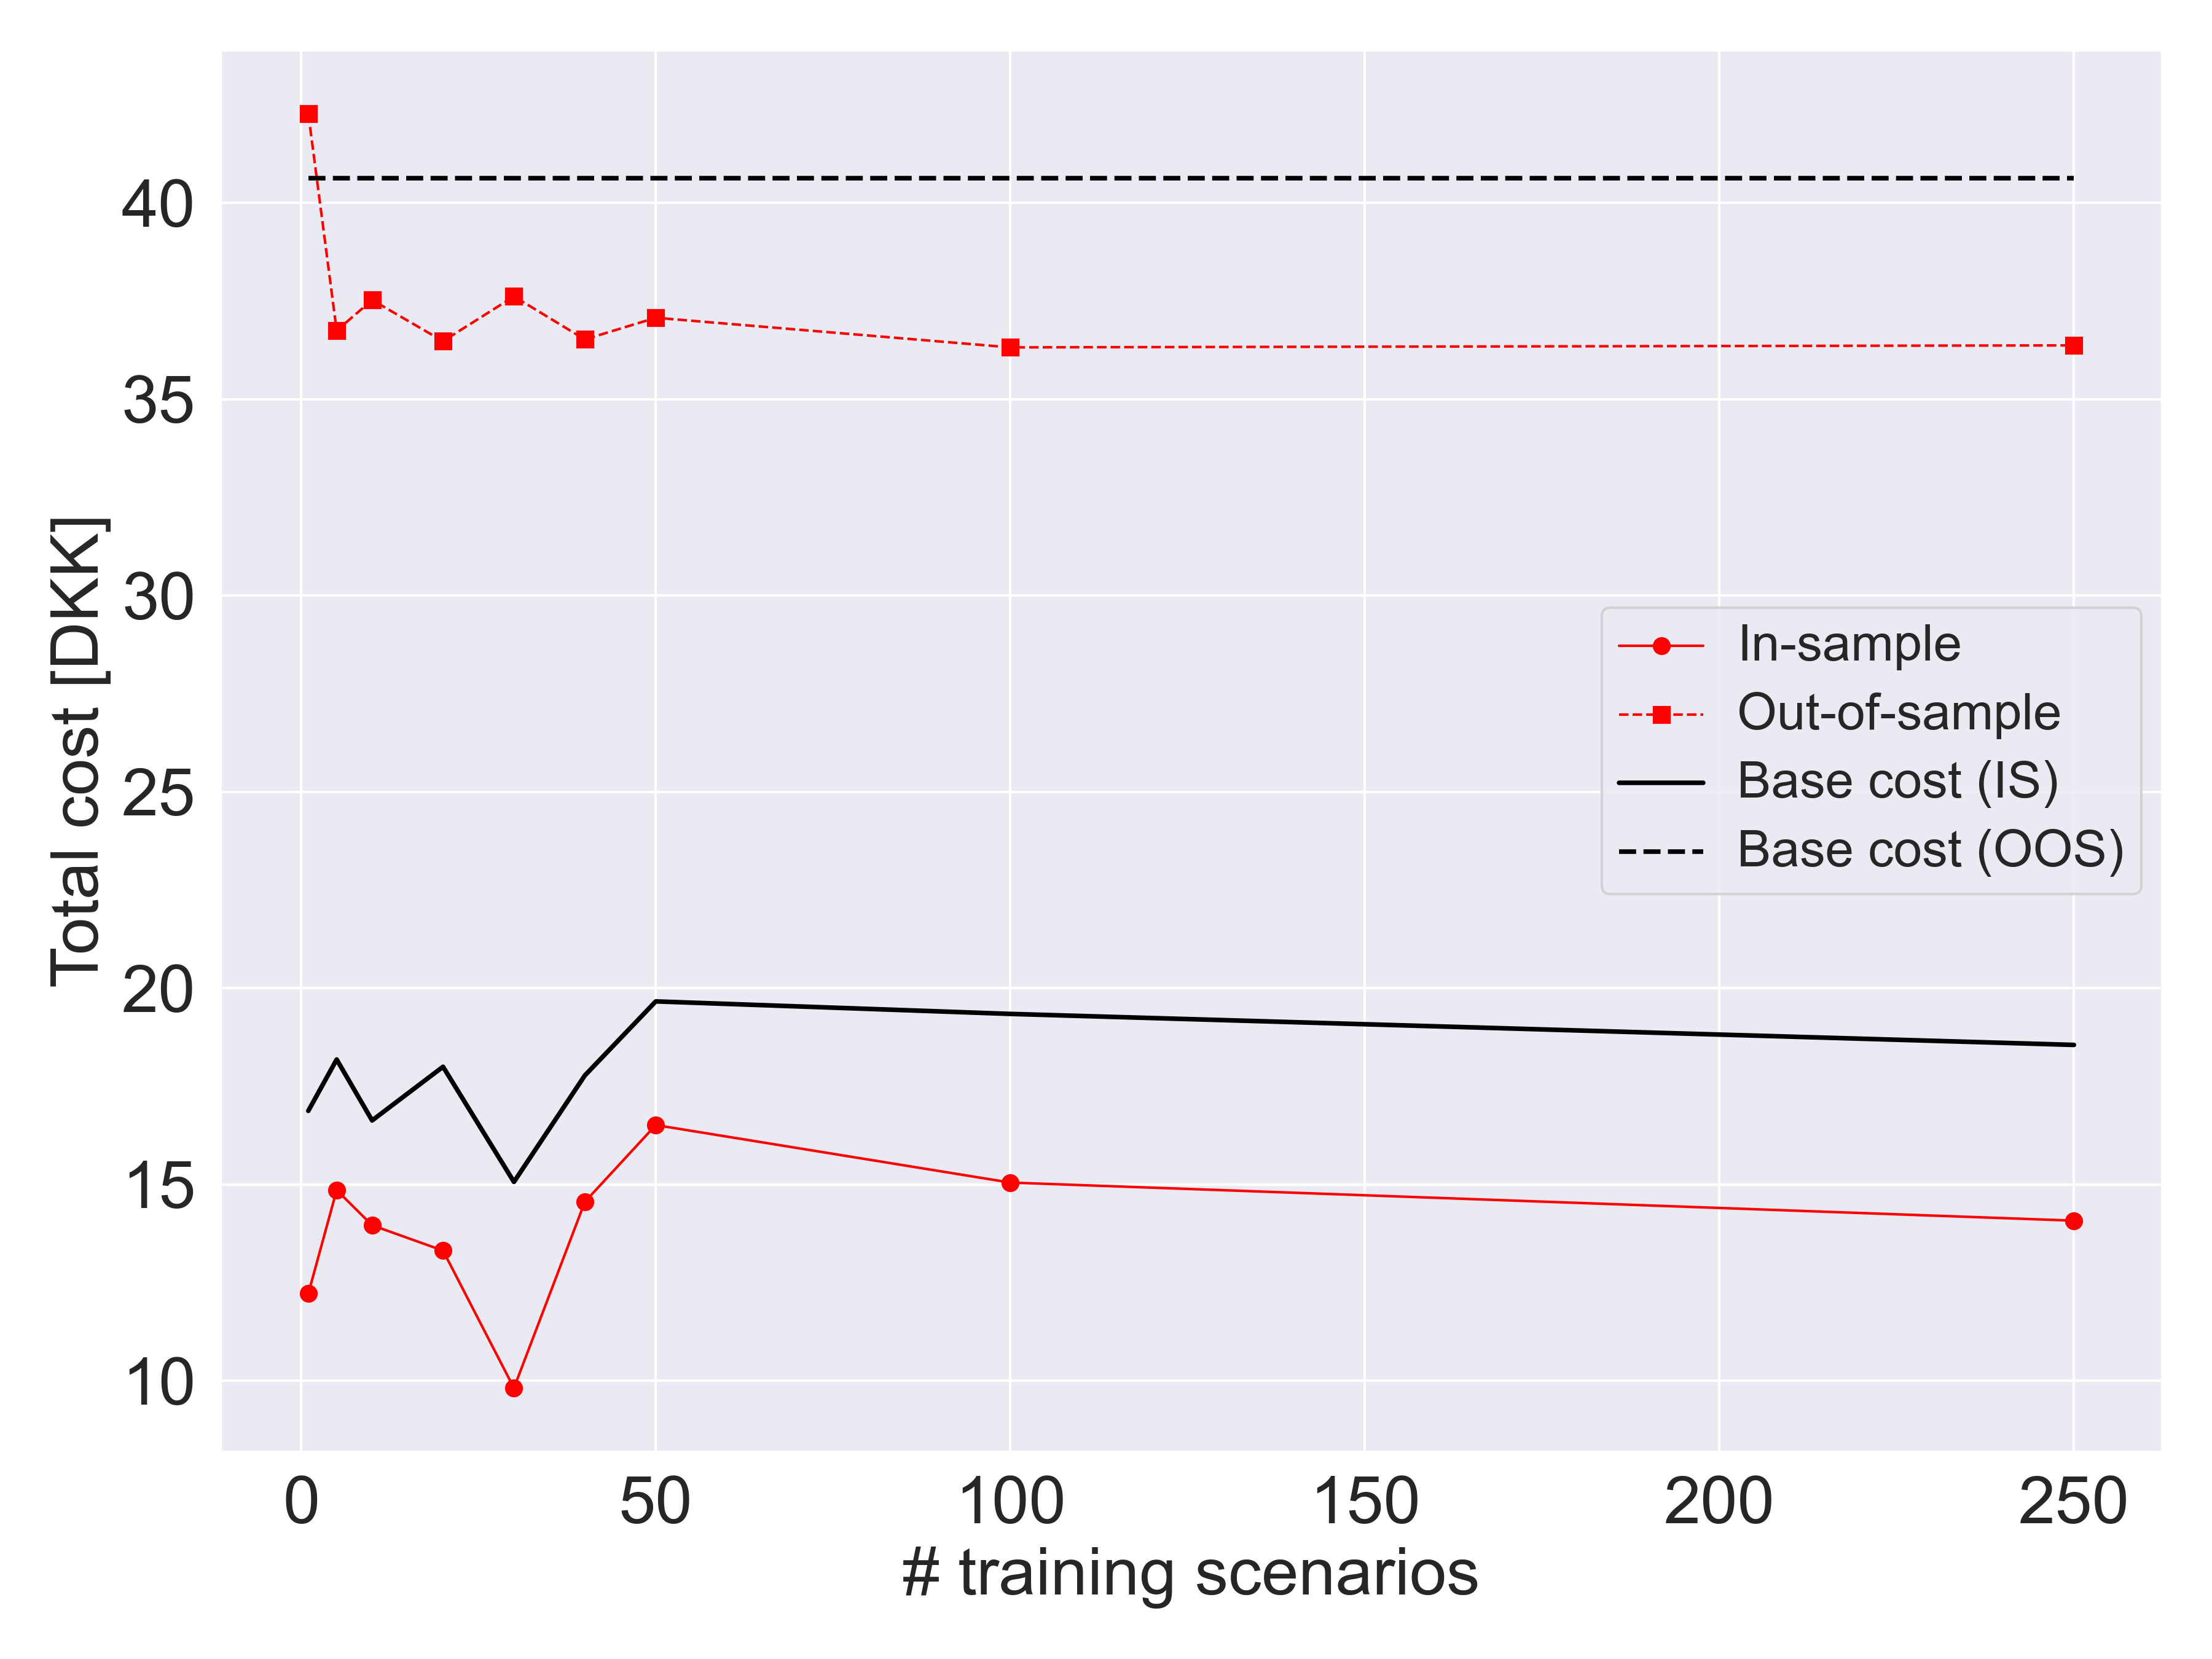
\includegraphics[width=\columnwidth]{../figures/admm_nb_scenarios_effect.png}
    \caption{Effect of number of IS scenarios on OOS performance for ADMM. Both are compared to the baseline costs of the freezer.}
    \label{fig:admm_nb_scenarios_effect}
\end{figure}

% \subsection{Lookback}

% TODO: create plot of effect of lookback parameter.
